\title{CS 311, Assignment 0}
% \subtitle{Hello}
\author{Harrithha (200010018), Shashank P (200010048)}

\date{\today}

\documentclass[12pt]{article}
\usepackage{fullpage}
\usepackage{enumitem}
\usepackage{amsmath,mathtools}
\usepackage{amssymb}
\usepackage[super]{nth}
\usepackage{textcomp}
\usepackage{hyperref}
\begin{document}
\maketitle

%---------------------------------------------------------------------
\section{Problem Statement}
This report describes the algorithmic approach used to achieve the motive of infiltrator during the course of progress from AC (Attacking Country) to DC (Defending Country) by varying different parameters like width, probability of Sensors being ON. Detailed analysis using various plots are also shown. 

%---------------------------------------------------------------------

\section{Approach \& Mathematical Modelling}
For solving the above problem, we take into account the position of the intruder and the 8 surrounding positions for analysis. The infiltrator moves only forward or remains at the same position. He moves when the sensor on his position is OFF and when any one of the sensors in the next row is OFF.

\begin{itemize}
    \item Let $p$ be the probability of getting a $heads$ on coin toss. Then, according to the question, if heads, the sensor is switched ON for the next 10 seconds. If tails, the sensor it switched OFF for the next 10 seconds.
    
    \item Let $w$ be the width that the infiltrator has to cross to reach the Defending Country.
    
    \item In the following diagrams for representation, R stands for $random$ configuration whose decision is taken based on the coin toss and F stands for $false$, i.e. the sensor is OFF.
    
\end{itemize} 
\\
At any given time $t$, the infiltrator can face one of these three situations : 
\begin{enumerate}

    \item Initially, when the infiltrator starts his/her attack, all the neighbouring sensors are OFF except the ones in the lowermost row, which is the first row of the border. The decision whether the sensors there will be ON/OFF will be taken based on the coin toss.
    
    The probability that the intruder moves forward in this situation is equal to the probability that at least one of the sensors in the next row is OFF, which is given by total minus the probability that all the 3 sensors in the next row are on with probability $p$.
    \vspace{50em}
    \begin{figure}[h]
    \centering
    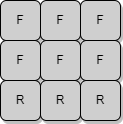
\includegraphics[width=0.25\textwidth]{Start.drawio.png}
    \caption{Start Configuration (1 time)}
    \label{fig:mesh1}
    \end{figure}
\[P(moving\: forward) = 1 - p^3\]
\begin{equation}
Number\: of\: steps = \frac{1}{1 - p^3}
\end{equation}

 \item Once the infiltrator enters the border, all the neighbouring sensors are configured according to the decision taken by coin toss.

The probability that the intruder moves forward in this situation is equal to the probability that the sensor at the position where the intruder is, is OFF which is given by $1 - p$ and at least one of the sensors in the next row is OFF, which is given by total minus the probability that all the 3 sensors in the next row are on with probability $p$.
   
   \begin{figure}[h]
    \centering
    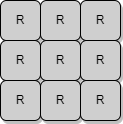
\includegraphics[width=0.25\textwidth]{Middle.drawio.png}
    \caption{General Configuration ($w$ - 1 times)}
    \label{fig:mesh1}
    \end{figure}

\[P(moving\: forward) = (1 - p)(1 - p^3)\]
\begin{equation}
Number\: of\: steps = \frac{w - 1}{(1 - p)(1 - p^3)}
\end{equation}

 \item Finally, when the infiltrator is in the bottom-most row of the border, all the sensors in the lowermost row are OFF(as no sensor exists there). The remaining sensors are configured according to the decision taken by coin toss.
 
 The probability that the intruder moves forward in this situation is equal to the probability that the sensor at the position where the intruder is, is OFF which is given by $1 - p$.
    \begin{figure}[t]
    \centering
    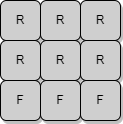
\includegraphics[width=0.25\textwidth]{End.drawio.png}
    \caption{End Configuration (1 time)}
    \label{fig:mesh1}
    \end{figure}
\[P(moving\: forward) = 1 - p\]
\[Number\: of\: steps = \frac{1}{1 - p}\]
\end{enumerate} \\
\textbf{FORMULA : } 
We will add (1), (2), (3) to get the total number of steps and multiply the entire expression by 10 as each step is taken in 10 seconds to get the total time required to cross from Defending to Attacking Country.

Therefore,
\begin{equation}
    Total\: time\: taken = \frac{10(1 - p - p^3 + w)}{(1 - p)(1 - p^3)}
\end{equation}

%---------------------------------------------------------------------

\section{Code Flow \& Execution}
We have created 6 code files which are as follows:
    \begin{itemize}
        \item Intruder.java - This models the infiltrator. It takes an argument as the width of the border and consists of two methods :
        \begin{enumerate}
            \item \textbf{move\_forward} : This increments the infiltrator's position by one for every move forward.
            \item \textbf{goal\_test} : This returns $true$ or $false$ depending upon whether the infiltrator has reached the Defending country or not.
        \end{enumerate}
        \item Border.java - This models the border. It takes as argument the width of the border $w$ and the probability $p$ of getting heads on the coin toss and consists of one method :
        \begin{enumerate}
            \item \textbf{get\_env} : This function returns the environment i.e. the information of the configuration of the 9 sensors at any given time as a 2D array.
        \end{enumerate} \newpage
        \item Main.java - It is the main file to be run and consists of two methods : \begin{enumerate}
            \item \textbf{can\_move\_forward} : Returns true or false depending upon whether the sensors at the position of the infiltrator is OFF and at least one of the 3 sensors in the next row is OFF or not.
            \item \textbf{main} : This is the main program which is used to model the movement of the infiltrator from the Attacking country to the Defending Country.
        \end{enumerate}
        \item Clock.java - This models the clock by initializing it to 0 and incrementing it by 10 seconds for each move made by the infiltrator

        \item Sensor.java - It models one sensor in the border. It has 2 methods: 
        \begin{enumerate}
            \item \textbf{set\_random\_state} : Sets whether the particular sensor is ON or OFF based on a coin toss with probability p.
            \item \textbf{get\_state} : This method returns the current state of the sensor, i.e., ON or OFF.
        \end{enumerate}
        
        \item analysis.ipynb - This is a well commented code base used to plot various graphs and compare the experimental and theoretical values of $p$ and $w$.
        
    \end{itemize}
Each file is embedded with a separate class which finally top inherits to \textbf{Main.java} file. We run a for loop for each $p$ and $w$ by passing it as a command line argument. The command line executions are: \\ \newline
$>>$ \textit{cd Scripts && javac Main.java && java Main {w} {p}} \\ \newline
The outputs for \textbf{analysis.ipynb} file are stored in $result.pkl$ file where for each combination of $w$, $p$ the average time of 10 runs is taken.

\section{Graphs}
The following graphs were plotted : 
\begin{enumerate}
    \item Figure 4 shows the graph and where we have used the parameters as follows:
   \begin{itemize}
        \item X-Axis: Probability
        \item Y-Axis: Time
   \end{itemize}

The graph shows that the formula we derived for total time taken (theoretical value) is almost same as the experimental results.
\begin{center}
    \begin{figure}[h]
        \centering
        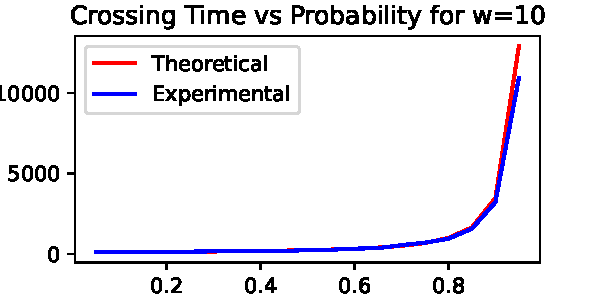
\includegraphics[width=10cm, height=4.5cm]{TvsP.pdf}
        \caption{Variation of Average time with Width}
    \end{figure}
\end{center}

\vspace{50em}
\item Figure 5 shows the graph and where we have used the parameters as follows:
   \begin{itemize}
        \item X-Axis: Width
        \item Y-Axis: Time
   \end{itemize}

The graph shows that the experimental variation of time with width is almost same as the theoretical results.
\begin{center}
    \begin{figure}[h]
        \centering
        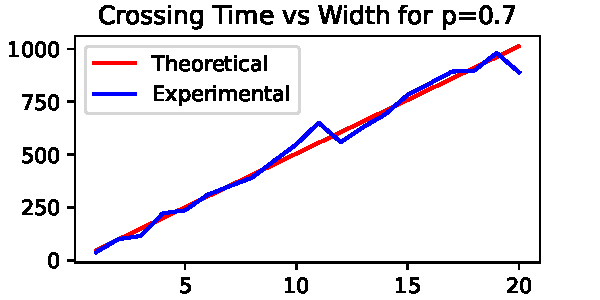
\includegraphics[width=10cm, height=4.5cm]{TvsW.pdf}
        \caption{Variation of Average time with Width}
    \end{figure}
\end{center}

\item Figure 6 shows the contour plot and where we have used the parameters as follows:
   \begin{itemize}
        \item X-Axis: Probability
        \item Y-Axis: Width
   \end{itemize}

The graph shows that the experimental variation of time with width and probability is almost same as the theoretical results.
\begin{center}
    \begin{figure}[h]
        \centering
        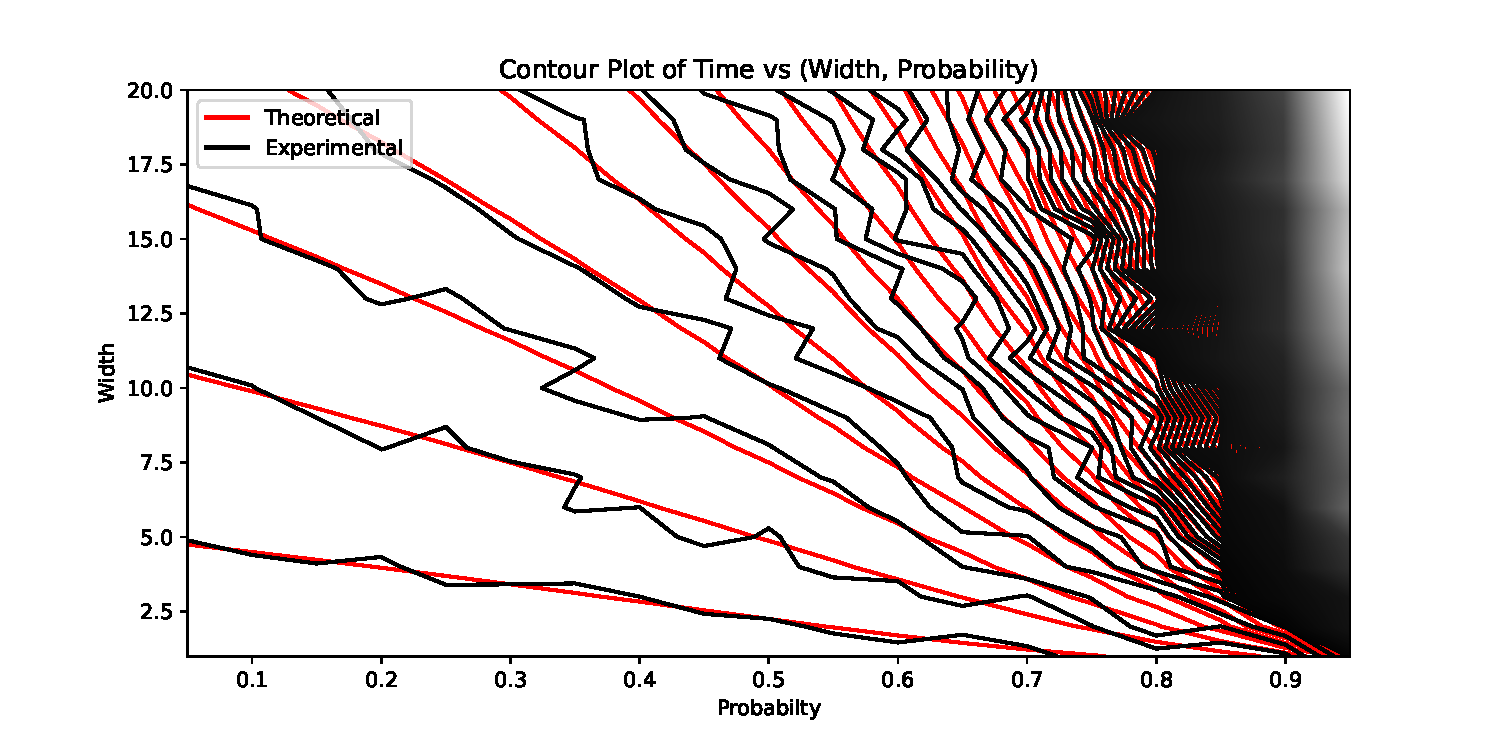
\includegraphics[width=15cm, height=6cm]{contour.pdf}
        \caption{Contour Plot of Time vs (Width, Probability)}
    \end{figure}
\end{center}

\item Figure 7 shows a 3D plot of experimental results, where we have used the following parameters :
   \begin{itemize}
        \item X-Axis: Width
        \item Y-Axis: Probability
        \item Z-Axis: Crossing Time (sec)
   \end{itemize}

\begin{center}
    \begin{figure}[h]
        \centering
        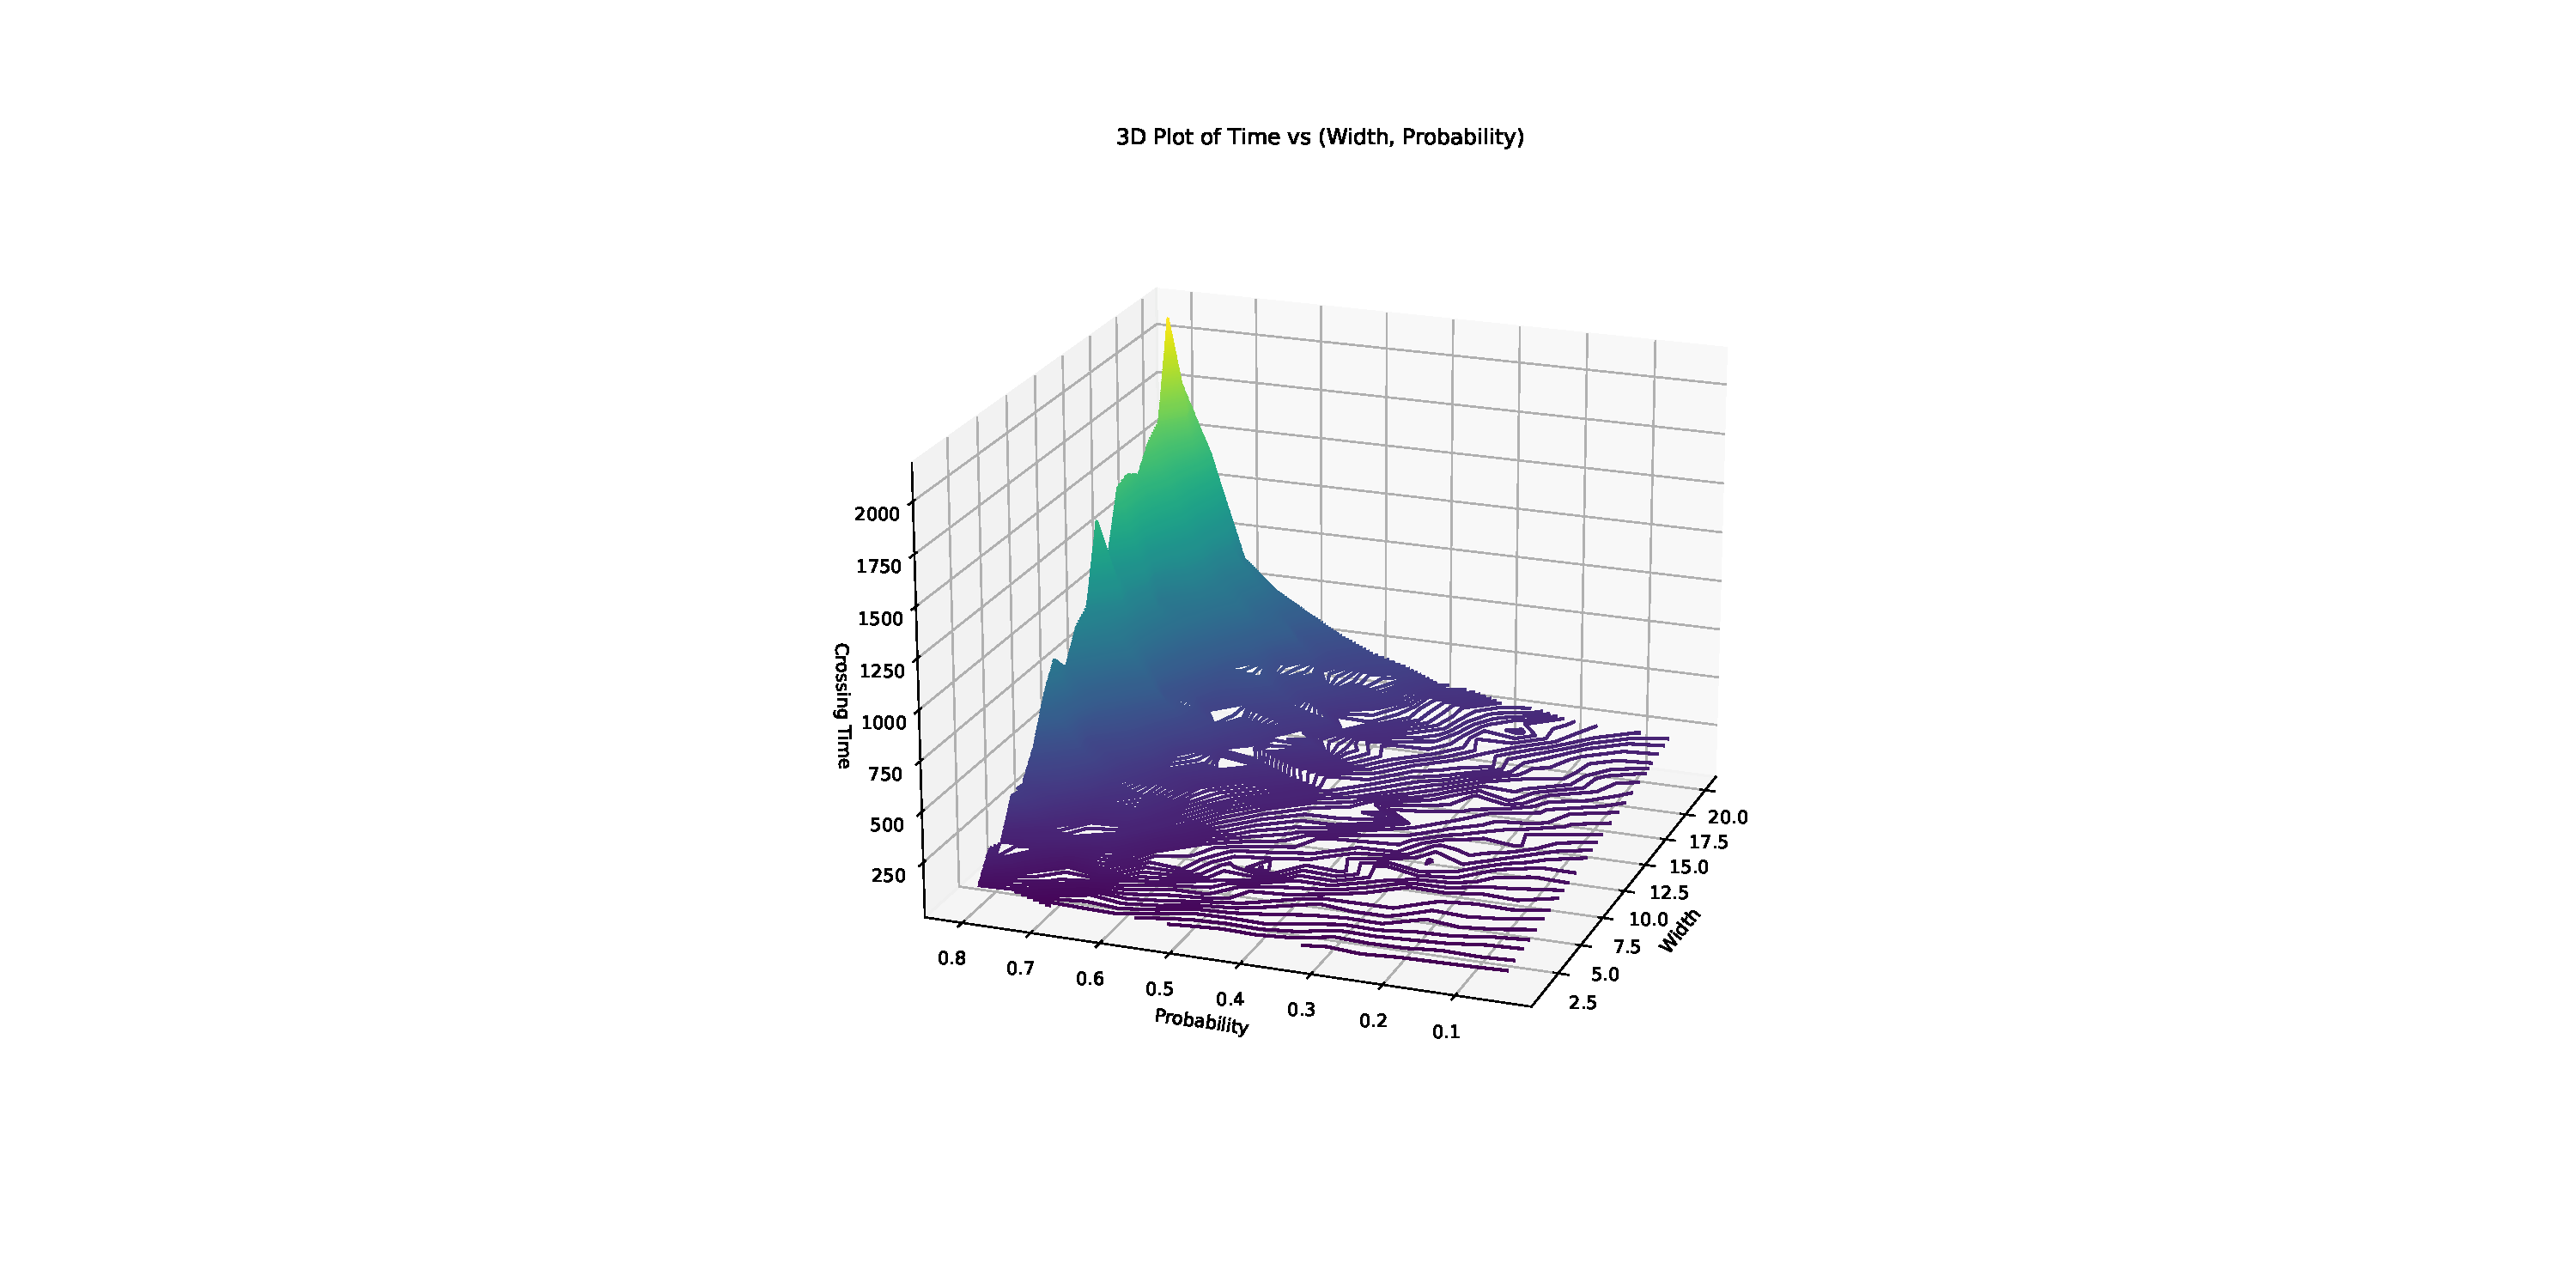
\includegraphics[width=17cm, height=8cm]{3D.pdf}
        \caption{3D Plot of Time vs (Width, Probability)}
    \end{figure}
\end{center}

\end{enumerate}
%---------------------------------------------------------------------
\section{Results \& Conclusions}
\begin{itemize}
    \item We have chosen P = \{0.05, 0.1,  0.15, 0.2, 0.25, 0.3, 0.35, 0.4, 0.45, 0.5, 0.55, 0.6, 0.65, 0.7, 0.75, 0.8, 0.85, 0.9, 0.95\}
    \item We have chosen W = \{1, 2, 3, 4, 5, 6, 7, 8, 9, 10, 11, 12, 13, 14, 15, 16, 17, 18, 19, 20\}
    \item \textbf{Effect due to variation in width} \\
    As the parameter $w$ (width) was increased, the time taken by the infiltrator to cross from Defending to Attacking Country is also increased. The reason behind that is that, the infiltrator will have to cover more distance with increasing value of width.
    \item \textbf{Effect due to variation of probability of sensors being ON} \\
    As the probability of sensors being ON increased, the time taken by the infiltrator to cross also increases. The reason behind that is that, as the probability of sensors being ON increases, the infiltrator's options to proceed towards Defending Country diminishes and hence time required will increase.
    \item \textbf{Comparison with theoretical results} \\
    As we can observe from graphs in the previous section, our theoretical formula derived is consistent with the experimental results.
\end{itemize}

%---------------------------------------------------------------------

\end{document}
